\chapter{Примеры использования и перспективы}

\TODO

\section{Визуализация броуновского движения}

\TODO

\section{Получение числа π методом Гальперина}\label{pipool}

Реализованную симуляцию можно использовать для вычисления числа \(\pi\)
методом Г.~Гальперина~\cite{poolpi}.
Этот метод заключается в том, что в системе из стенки слева,
тела массой \(1\) и телом массой \(100^{n - 1}\) эти тела соударяются и число этих столкновений
будет равно первым \(n\) цифрам числа~\(\pi\)~\cite{habrpi}.
При этом, в системе нет трения, т.е. сталкиваться тела закончат, когда оба улетят вправо, причём у тела с меньшей массой скорость будет меньше.
Разработанный движок хоть и рассчитан на движение с трением, но может и без него, если коэффициент трения сделать равным нулю.

Например, рассчитать первые 4 цифры можно следующим образом.
Очистить модель, поставить воспроизведение на паузу и отмотать время в ноль~(рисунок~\ref{pistep1fig}).

\begin{figure}[H]
    \centering
    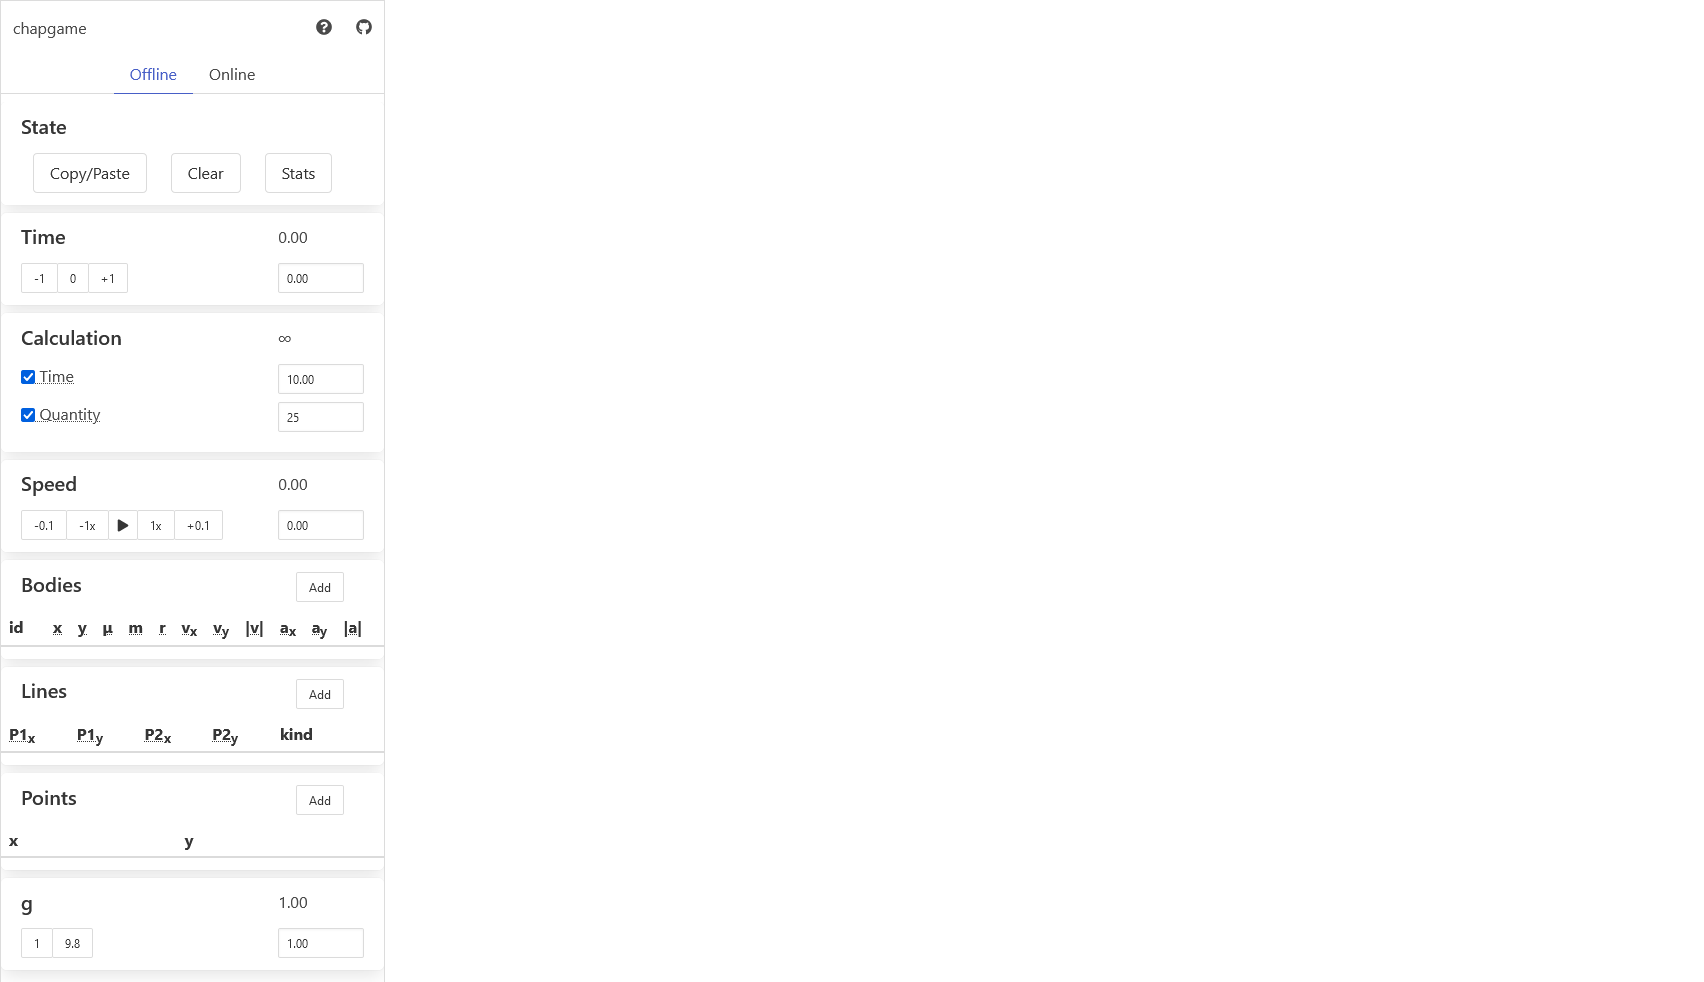
\includegraphics[width=15cm]{pistep1}
    \caption{Шаг 1\label{pistep1fig}}
\end{figure}

Добавить вертикальную линию, которая будет располагаться слева от тел~(рисунок~\ref{pistep2fig}).

\begin{figure}[H]
    \centering
    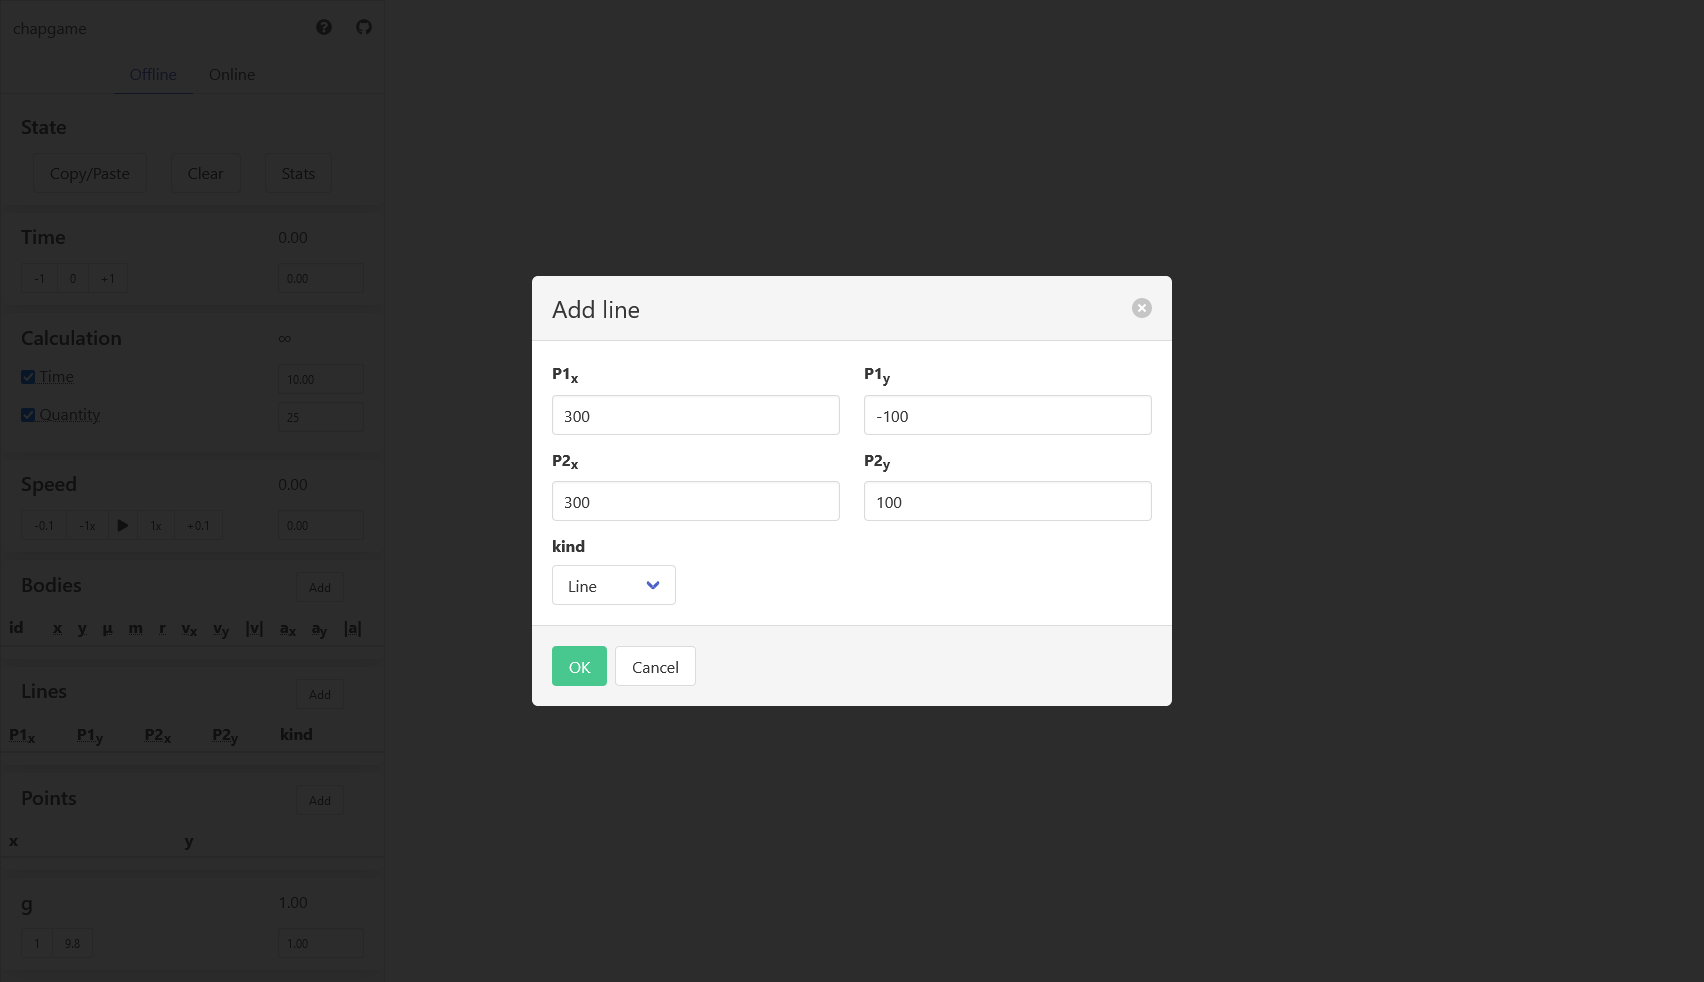
\includegraphics[width=15cm]{pistep2}
    \caption{Шаг 2\label{pistep2fig}}
\end{figure}

Добавить тело с меньшей массой~(рисунок~\ref{pistep3fig}).
Так как оно должно быть правее добавленной линии, координата по оси \(X\)
добавляемого тела должна быть больше.

\begin{figure}[H]
    \centering
    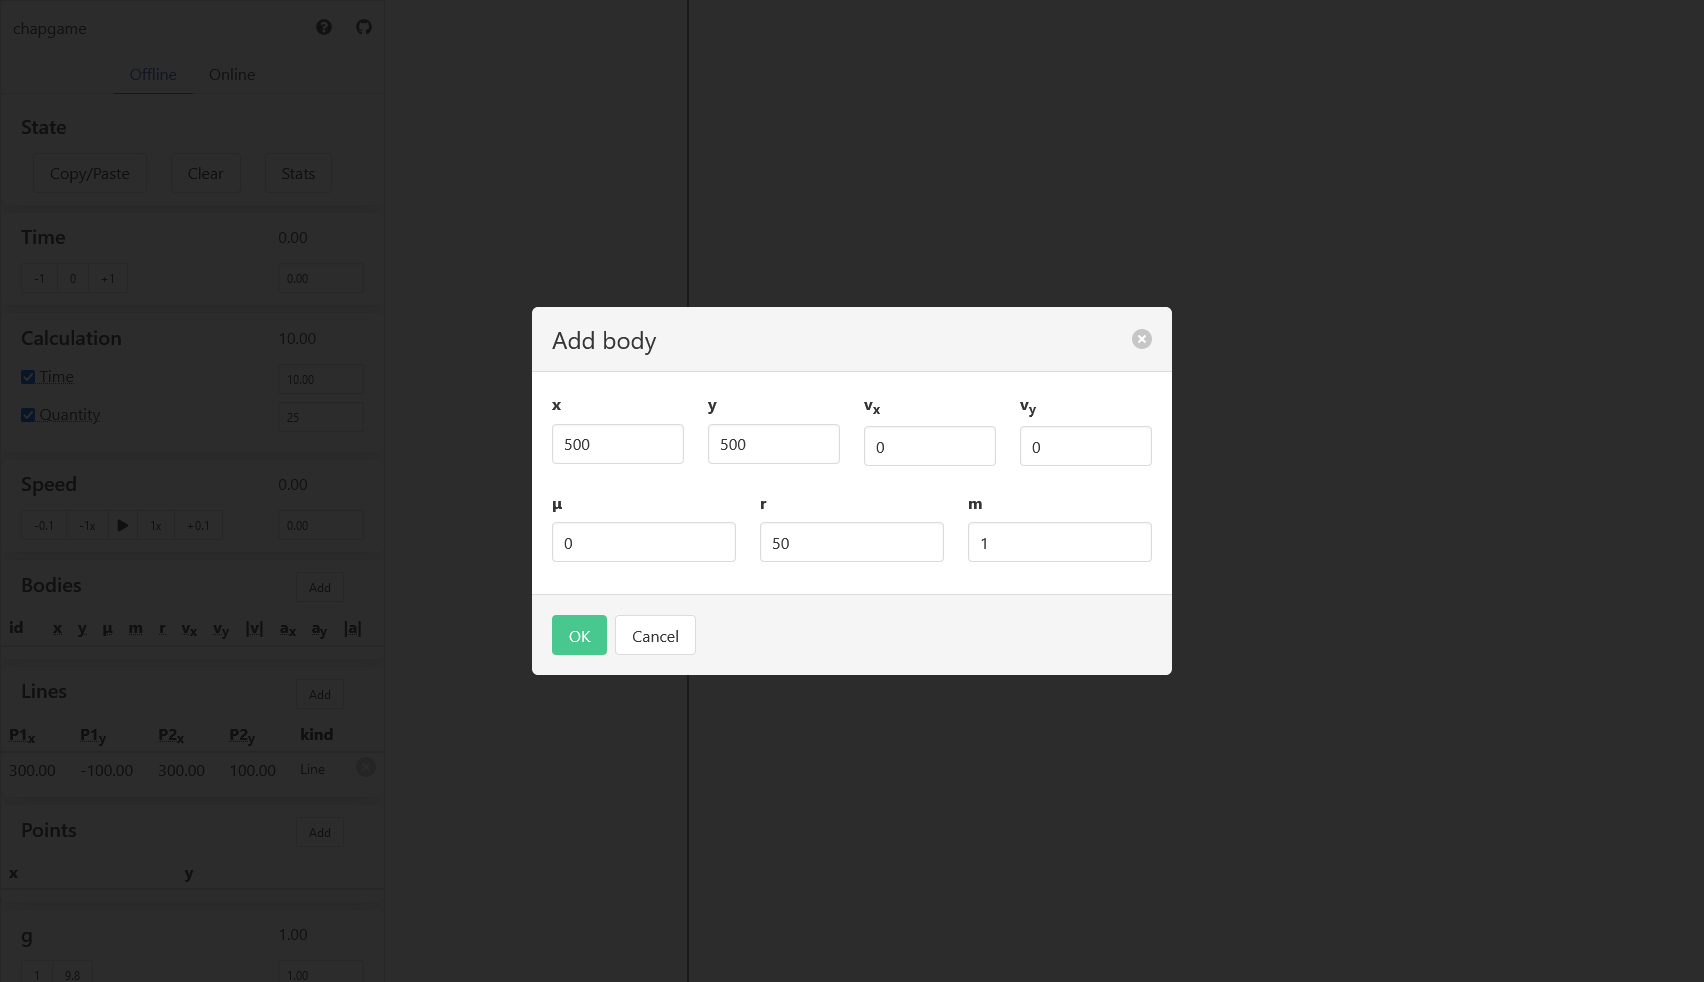
\includegraphics[width=15cm]{pistep3}
    \caption{Шаг 3\label{pistep3fig}}
\end{figure}

Добавить тело с большей массой, его координата по оси \(X\) должна быть ещё больше;
радиус можно оставить таким же, а масса должна быть в \(100^3\) раз больше так как требуется вычислить 4 цифры;
скорость этого тела должна быть направлена влево (рисунок~\ref{pistep4fig}).

\begin{figure}[H]
    \centering
    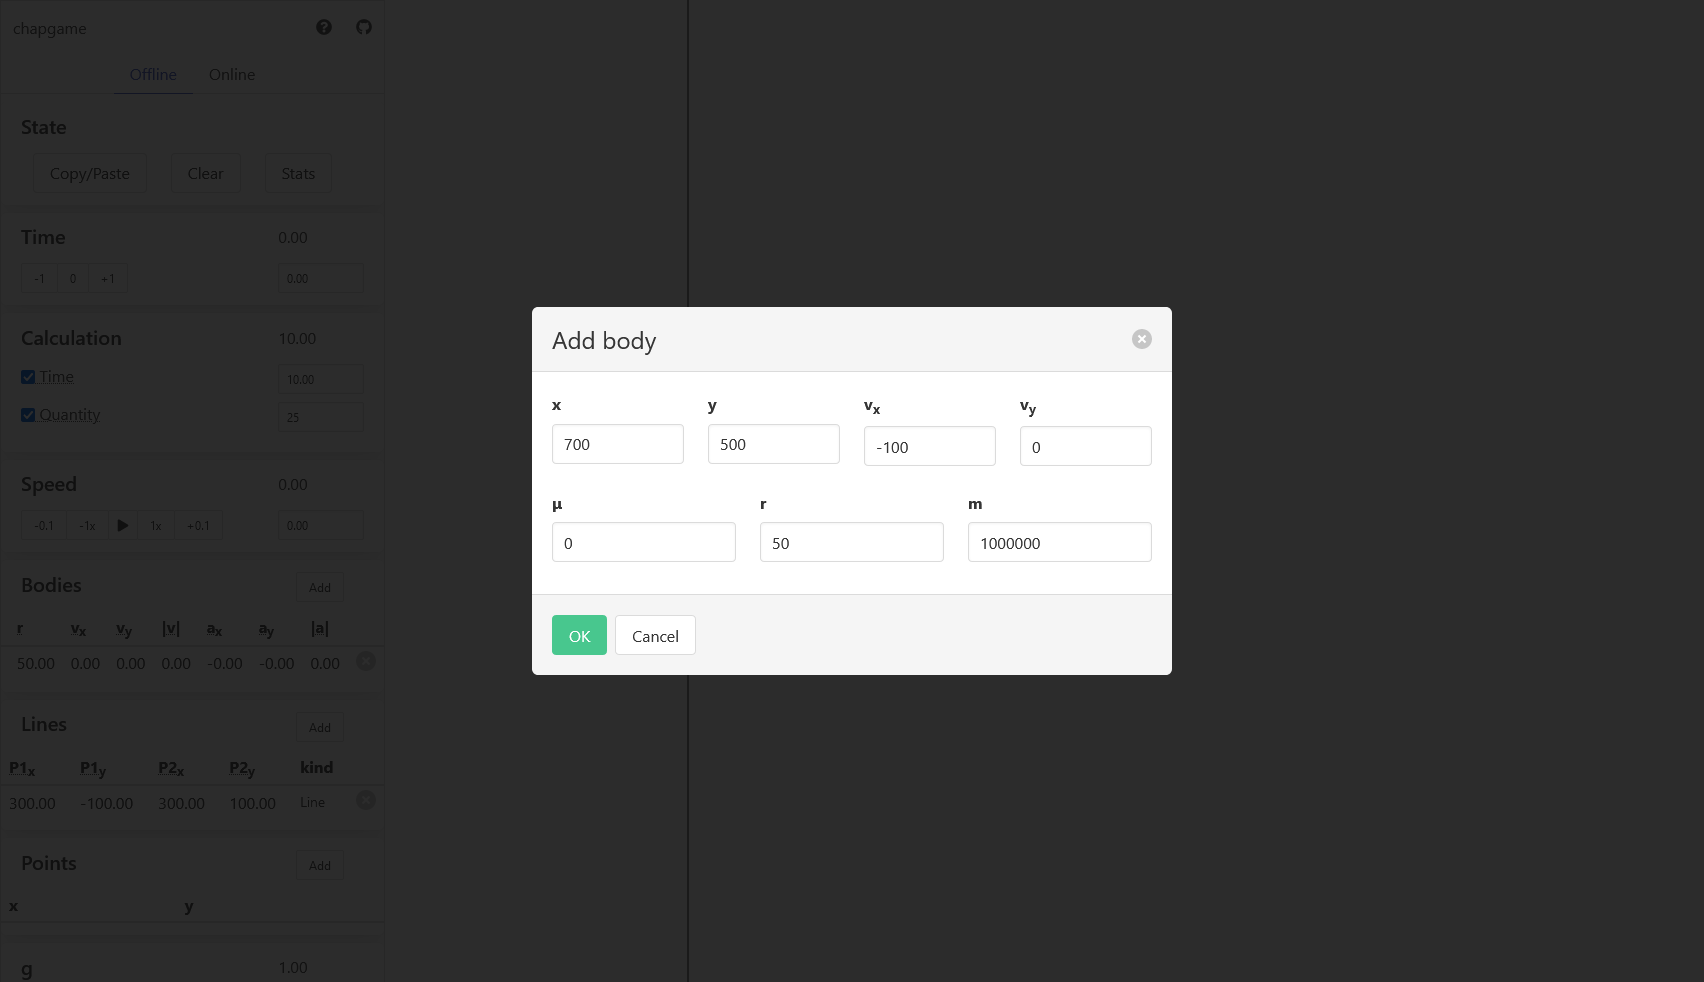
\includegraphics[width=15cm]{pistep4}
    \caption{Шаг 4\label{pistep4fig}}
\end{figure}

Убрать галочки, отвечающие за параметры расчёта, чтобы модель рассчиталась до конца~(рисунок~\ref{pistep5fig}).

\begin{figure}[H]
    \centering
    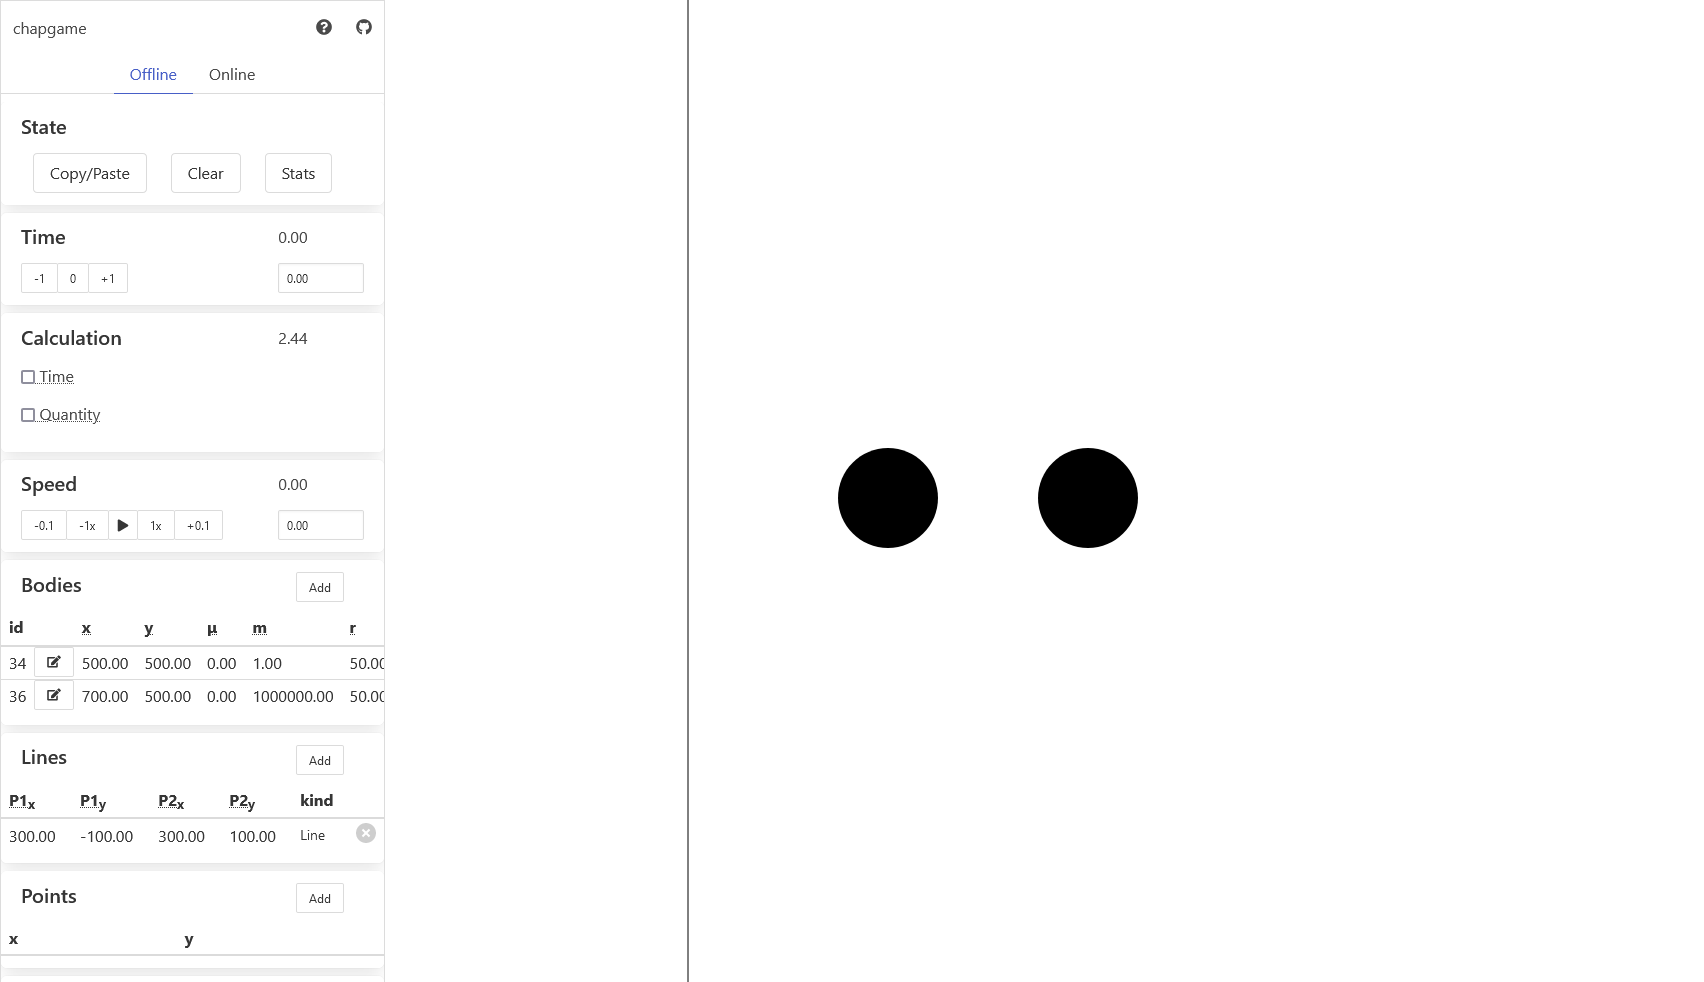
\includegraphics[width=15cm]{pistep5}
    \caption{Шаг 5\label{pistep5fig}}
\end{figure}

Снять воспроизведение с паузы и дождаться когда произойдёт расчёт. Можно наблюдать за столкновениями,
или сразу открыть статистику и в счётчике столкновений будет искомое число: \(3141\), что является
первыми 4 цифрами числа \(\pi \approx 3.14159265359\).

\begin{figure}[H]
    \centering
    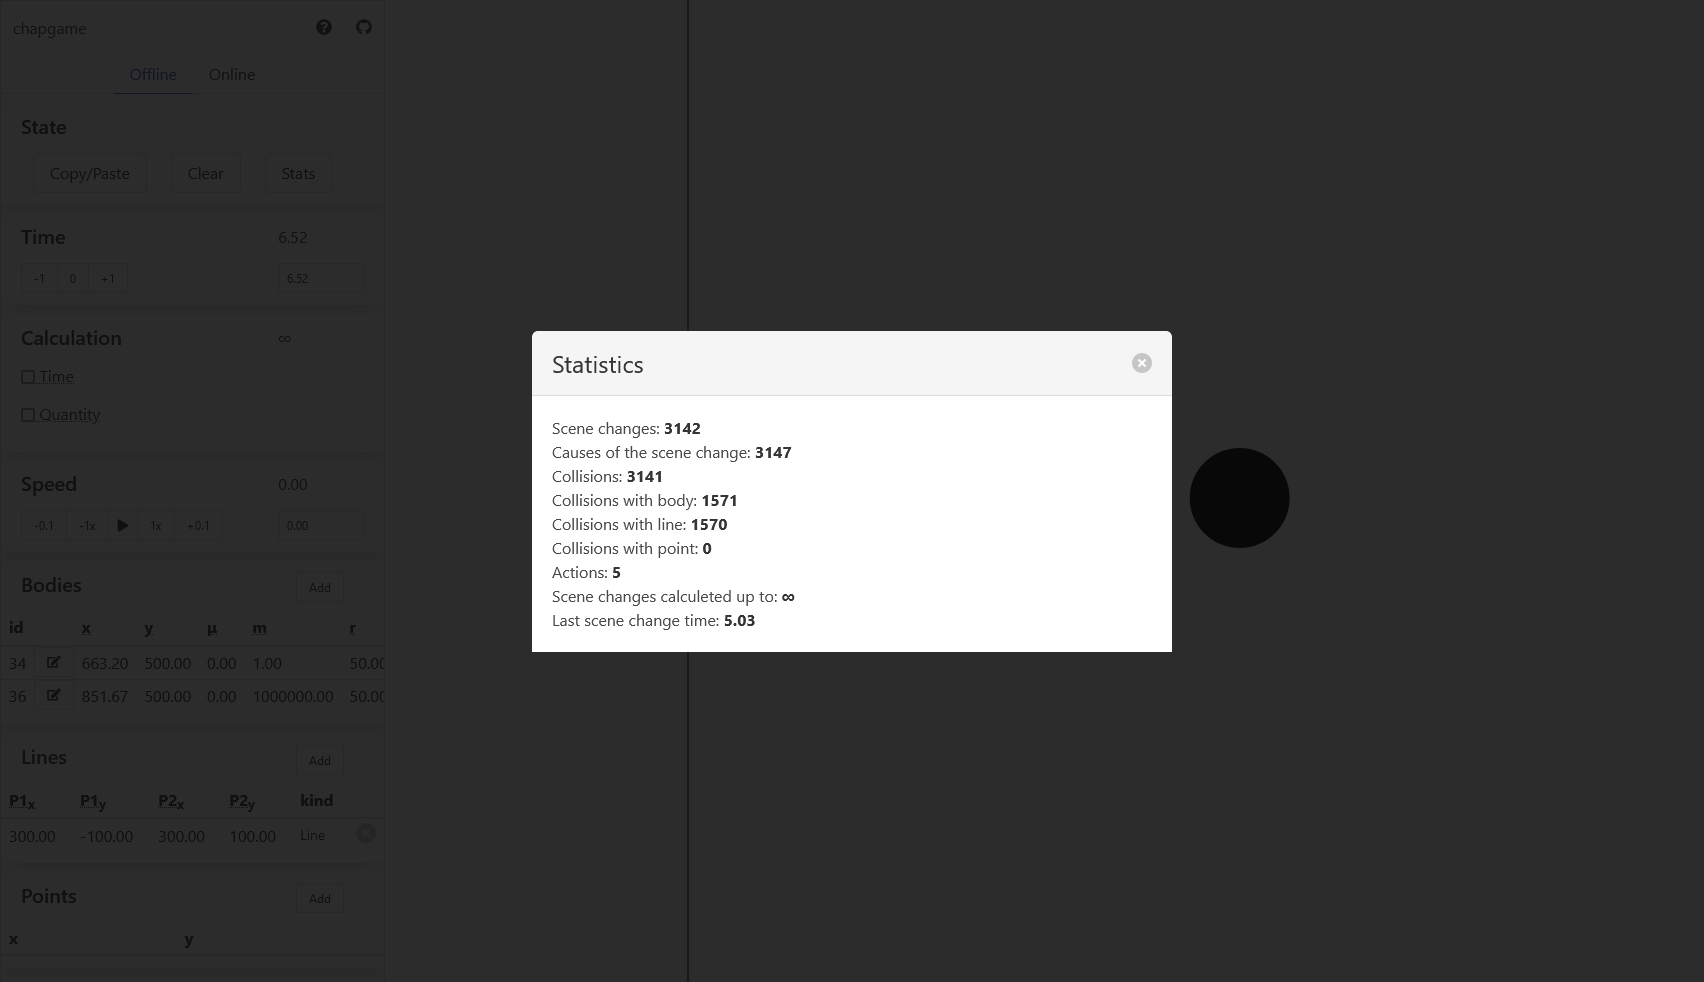
\includegraphics[width=15cm]{pistep6}
    \caption{Шаг 6\label{pistep6fig}}
\end{figure}

\TODO https://habr.com/ru/post/533454/

\section{Перспективы и дальнейшее возможное развитие}

\subsection{Расширение возможностей многопользовательского режима}

\TODO Сохранение реплеев на сервере, чат.

\subsection{Клон игры <<Смешарики>> (может быть известна как <<Чапаев>>)}

\TODO https://shararam.fandom.com/wiki/Смешарики\_(игра)

\subsection{Оптимизация}

\TODO мемоизация и т.д.
Профилирование. Поиск плохих мест в алгоритме.

\subsection{Распараллеливание}

\TODO domainslib

\subsection{Обобщение \TODO}

\TODO Воздействие нескольких сил, неупругие столкновения,
применение действий при взаимодействии или даже трёхмерное пространство и т.д.

% \subsection{Формальная верификация частей алгоритма}

\TODO
